% !TEX root = ../thesis_main.tex
\chapter{Theory and state of the art}\label{chap:theory}
This chapter will provide a basis for understanding the principles on which this work is based as well as the phenomena used in the different builds. It will cover many aspects, but of course, a deeper understanding can be gained by also consulting the references mentioned. At first, the quantum mechanical approach describing nuclei and spin systems will be given followed by a more 
    \section{Nuclei and Spins}
        \label{theory:section:nucleiSpins}
        The postulation of an electron spin in 1926 \ref{} and later, in 1928, of a proton spin \ref{} opened
        up new areas of research.\todo{more history}
        Each particle has magnetic properties to which both electrons and the nucleus, i.e. protons and neutrons, conribute. We consider the electons' contributions to be of a static nature because of the fast movement (see \ref{chemical shif, kann man so sagen?}) and instead turn to the nucleus' magnetic properties. As we want to manipulate nuclei electromagnetically, their magnetic momentum is the relevant physical property in this case.
        The magnetic momentum $\vec M$ of a nucleus is connected to the spin $\vec S$ by the gyromagnetic ratio $\gamma$, a nucleus specific proportionality factor \cite{balanis_advanced_nodate}:
        \begin{equation}
            \vec M = \gamma \vec S
            \label{eq:gyromagneticRatio}
        \end{equation}
        The spin can be described as and seems to behave like an angular momentum, but is not created by a particle rotation but rather an inrinsic property of the particle. Each of the nuclei, in case of the hydrogen nucleus also simply called "spin" as it is only a single proton and thus a single spin, is described by the quantum numbers according to the quantized angular momenta, using quantum numbers I and m. We consider the protons and neutrons to be in their spin $\tfrac{1}{2}$ state in all cases considered here, only at very high energies in the \SI{}{\giga\electronvolt}, other states can occur. The quantum numbers are described by the quantum operators   The nucleus thus has m~=~(2I~+~1) energy eigenstates that are degenerated in zero field. If a magnetic field is present though, the energy levels will split with energy differences proportional to the magnetic field strength, the Zeeman energy splittings.
        \subsection{Zeeman energy splitting}
            If a particle with a spin $S\neq 0$ is exposed to a magnetic field $B_0$, it experiences an energy splitting of its eigenstates due to the fact that the direction of the spins compared to the field is now a relevant parameter for the overall energy of the particle. Both the gyromagnetic ratio and the field strength determine how big that splitting is:
            \begin{equation}
                E_{Z} = -\gamma m B
            \end{equation}
            where $E_Z$ is the zeeman energy difference to the non-split state and m is the magnetic quantum number \cite{gerlach_experimentelle_1989, bloch_nuclear_1946}. The negative sign implies that a antiparallel orientation with the field for particle with positive $\gamma$ is energetically favorable. For example, $^1$H and $^{15}$N, the two main nuclei considered in this work, show energy splittings into two levels ($2\cdot\tfrac{1}{2}+1$), but of about a factor of 10 stronger for $^1$H due to the by that factor larger gyromagnetic ratio. (see figure \ref{figure:theory:zeemanSplittings}).
            \begin{figure}
                \centering
                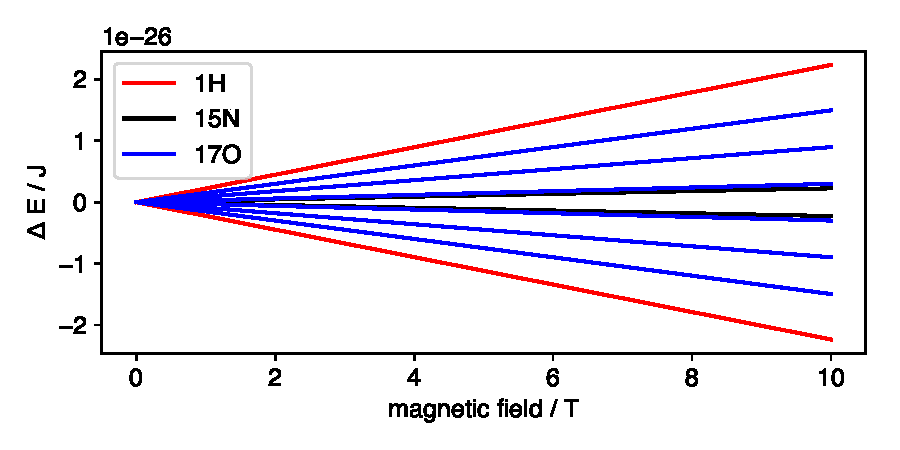
\includegraphics[width=0.9\textwidth]{/figures/theory/zeemanPlot.pdf}
                \caption[Zeeman energy splitting]{The Zeeman energy splittings of three nuclei over magnetic field. Note the difference in slopes for the spin $\tfrac{1}{2}$ nuclei 1H and 15N caused by the different gyromagnetic ratios. Arbitraily, 17O, a spin $\tfrac{5}{2}$ nucleus, was plotted to visualize higher order splittings with $2 \cdot\tfrac{5}{2}+1 = 6$ energy levels. }
                \label{figure:theory:zeemanSplittings}
            \end{figure}
            Individual spins can be described by their angular momentum operators $\hat{I}_x$, $\hat{I}_y$ and $\hat{I}_z$ that return the eigenvalue of the state in its respective direction \cite{pauli_zur_1988}. For the z direction, an additional quantum number S is defined by setting the external field up in z direction without loss of generality:
            \begin{equation}
                \hat I_z \ket{I, S} = S \ket{I,S}
            \end{equation}
            Considering a spin-1/2 particle in a magnetic field along the z-axis (e.g. the proton as a prominent particle in NMR), these eigenstates are
            \begin{equation}
            \ket\alpha = \begin{pmatrix}1\\0\end{pmatrix} \hspace{2 cm} \ket\beta =
            \begin{pmatrix}0\\1\end{pmatrix}
            \end{equation}
            with the eigenvalues of $\pm 1/2$.  Generally, every spin-1/2 particle can be in any superposition of those two eigenstates:
            \begin{equation}
                \ket\psi = c_\alpha \ket\alpha + c_\beta \ket \beta = \begin{pmatrix} c_\alpha \\
                c_\beta\end{pmatrix}
            \end{equation}
            These superposition states evolve under external conditions until a eigenstate of the particle
            is reached. Generally, a sample does not consist of one, but of many nuclei and thus many spins need to be
            described to describe the system. To do so, usually the density matrix formalism is introduced.
            It onsiders an ensembe of spins that do not interact with each other. In this case, the
            expectation value of an operator for a single spin $\braket{\hat Q}$ is given by 
            \begin{equation}
            \bra\psi\hat Q\ket\psi = \left( c_\alpha^*, c_\beta^*\right)
            \begin{pmatrix}
                Q_{\alpha\alpha} Q_{\alpha\beta}\\
                Q_{\beta\alpha} Q_{\beta\beta}
            \end{pmatrix}
            \begin{pmatrix}
                c_\alpha\\
                c_\beta
            \end{pmatrix}
            \end{equation}
            as shown in \cite{sakurai_modern_2017}. It can be shown that this is equal to the trace of the density operator
            $\ket\psi\bra\psi$ multiplied with said operator \cite{levitt_spin_nodate}
            \begin{equation}
                \braket{\hat Q} = \Tr \left\{\ket\psi\bra\psi\hat Q\right\}
            \end{equation}
            The states of the single spin can be described fully by the Pauli matrices $\vec{I} = \left\{ \hat{I_x}, \hat{I_y}, \hat{I_z}\right\}$
            \begin{align*}
                \vec I^2 \ket{j,m} &= j(j+1)\ket{j,m}\\
                \hat{I}_z \ket{j,m} &= m\ket{j,m}\\
                \hat{I}_\pm \ket{j,m} &= \sqrt{j(j+1)-m(m+1)}\ket{j,m\pm1}
            \end{align*}
            where $ \hat{I}_\pm = \hat{I}_x\pm i \hat{I}_y$.

            For multiple spins, it follows that the observable becomes the sum of their individual
            observables:
            \begin{equation}
                \braket{\hat Q_{all}}= \bra{\psi_1}\hat Q\ket{\psi_1} + \bra{\psi_2}\hat Q\ket{\psi_2} + \hdots =
                \Tr{\left\{\left(\ket{\psi_1}\bra{\psi_1} + \bra{\psi_2}\ket{\psi_2}+ \hdots \right) \hat Q\right\}}
            \end{equation}
            This means that the system of spins can be described by the sum of the density operators called
            the density matrix
            \begin{equation}
                \hat\rho = \overline{\ket\psi\bra\psi}.
            \end{equation}
            For a spin-1/2 ensemble, the density matrix in thermal equilibrium is
            \begin{equation}
                \hat \rho = \begin{pmatrix} \frac{1}{2}+\frac{1}{4}\mathbb{B}& 0\\ 0&
                \frac{1}{2}-\frac{1}{4}\mathbb{B}\end{pmatrix} = \frac {1}{2} \hat1 + \frac{1}{2} \mathbb{B}
                \hat I_z
            \end{equation}
            with $\mathbb{B} = \frac{\hbar\gamma B_0}{k_b T}$. That means that in thermal equilibrium, the
            non-diagonal elements are zero, i.e. the socalled coherences (off-diagonal elements) are all
            equally populated while there is a slight overpopulation of one of the two states. Through deflection from that
            equilibrium, coherences are populated as described in the following section.
        \subsection{Radiofrequency pulses}
            Using the density matrix formalism, radiofrequency pulses described by rotational operators can be
            applied to the whole ensemble. A pulse $\hat R_\phi(\beta)$ of phase $\phi$ (corresponding
            to the axis around which magnetization is rotated) and angle $\beta$ where
            $\beta=\omega_{nut} \cdot \tau_p$ exerting on a state $\ket\psi$ is described by 
            \begin{equation}
                \ket{\psi_\tau}= \hat R_\phi(\beta)\ket\psi
            \end{equation}
            Calculating the density matrix now leads to
            \begin{equation}
                \hat {\rho_\tau} = \overline{\ket{\psi_\tau}\bra{\psi_\tau}} = \overline{\hat
                    R_{\phi}(\beta)\ket\psi\bra\psi \hat R_\phi(-\beta)}
            \end{equation}
            where the overbar describes the averaging over all spins in the ensemble \cite{popov_modern_1990, chizhik_magnetic_2014}
            Finally, as we are considering the same flip angle for every single spin in the ensemble,
            the formula can be reduced to
            \begin{equation}
                \hat\rho_\tau = \hat R_\phi(\beta) \hat \rho \hat R_\phi(-\beta)
            \end{equation}
            meaning a rotation of the magnetization corresponds to a rotation of the desity matrix.
            If we consider a $\SI{90}{\degree}$ pulse around the x axis on the previously described
            equilibrium for a spin-1/2 ensemble it follows \cite{hosur_scaling_1990, levitt_spin_nodate}:
            \begin{equation}
                \begin{split}
                    \hat\rho_\tau = \hat R_x(\pi/2)\hat\rho\hat R_x(-\pi/2) &= \frac{1}{2} \hat 1 +
                    \frac{1}{2} \mathbb{B}\hat R_x(\pi/2) \hat I_z \hat R_x(-\pi/2)\\
                    &=
                    \begin{pmatrix}
                        \frac{1}{2} & -\frac{1}{4i}\mathbb{B}\\
                        \frac{1}{4i}\mathbb{B}\ & \frac{1}{2}
                    \end{pmatrix}
                \end{split}
            \end{equation}
            It can be equally shown that a $\SI{180}{\degree}$ pulse inverts the populations of the
            diagonal elements while the coherences are untouched.
            If the system is not in thermal equilibrium, the states will evolve and generally relax back
            into the original equilibrium state. If one neglects said relaxation at first, the evolution
            can be described by \todo{ref formula rotationg frame}
            \begin{equation}
                \begin{split}
                    \ket\psi_\upsilon &= \hat R_z(\Omega^0\upsilon)\ket\psi_\tau ~ \mathrm{and} \\
                    \hat\rho_\upsilon &= \hat R_z(\Omega^0\upsilon)\hat\rho_\tau\hat
                    R_z(-\Omega^0\upsilon)
                \end{split}
            \end{equation}
            which shows that only a time dependent phase $\exp{(\Omega^0 \upsilon)}$ is added to the coherences and the populations
            stay constant. This confirms the macroscopic observation that the ensemble of spins behaves like a rotating vector of
            magnetization in the x-y-plane (w\textbackslash o relaxation).
            If relaxation is added to the scheme, we can differentiate between relaxation of the
            coherences ($T_2$ relaxation) and that of the states ($T_1$ relaxation). The former affects
            the non diagonal elements only which will deacy to zero while the latter brings the populations of the states back to
            thermal equilibrium. That can be expressed by
            \begin{equation}
                \rho_{ij, \upsilon} = \rho_{ij, \tau} \exp{(\pm
                    i\Omega^0-\lambda)\upsilon},~\mathrm{i,j~=~
                1,2(+)~or~2,1(-)}
            \end{equation}
            for the non diagonal elements and
            \begin{equation}
                \rho_{ii,\upsilon} = (\rho_{ii,\tau} - \rho_{ii}^{eq})\exp(-\tau/T_1)+\rho_{ii}^{eq}
            \end{equation}
            for the diagonal elements \cite{levitt_spin_nodate}.
        \subsubsection{Signal detection}
        The signal induced into the receive coil of a scanner (sec. \ref{section:matMeth:rfPulses}, \ref{section:matMeth:receiveCoil} for hardware details) is described by the expectation value of the $\hat{I}_+$ operator \cite{levitt_spin_nodate}:
        \begin{equation}
            S(t) = \left< \hat{I}_+ \right> = tr\left(\sigma(t)\hat{I}_+\right)
        \end{equation}
        In addition to the pure signal, there will also a contribution of noise to the overall signal. This contribution will be arbitraryly distributed for 
        \subsection{Multiple spin ensembles}
            The description above was all related to a single kind of spin, but can - and has to - be extended to describe more complex systems containing multiple, interacting spins. To do so, the product operators, product states and product density matrices of all operators and states need to be calculated. This can be done by expanding the operators up to the necessary dimenion that is given by the N operators:
            \begin{equation*}
                A^p_n = \mathbb{I}_0\otimes\mathbb{I}_1\cdots \mathbb{I}_{n-1} \otimes A_n \otimes \mathbb{I}_{n+1}\cdots \mathbb{I}_N
            \end{equation*}
            where $\mathbb{I_i}$ is the unity matrix of operator $A_i$. The product operators have the advantage of making normal matrix multiplications possible where otherwise, kronecker products were needed \cite{green_theory_2012-1}:
            \begin{equation}
                A_n\otimes A_m = (A_n \otimes \mathbb{I}_m)(\mathbb{I}_n \otimes A_m) = A^p_nA^p_m
            \end{equation}
            Note that this is an especially convenient way of noting but will also cover coupling effects in the off-block-diagonal elements\todo{check again!}. Similarly, the extended states are established as kronecker products of their single states:
            \begin{equation}
                \ket{a_1,a_2, \dots, a_N} = \ket{a_1}\otimes\ket{a_2}\otimes\dots\otimes\ket{a_N}
            \end{equation}
            with all N substates and their respective quantum numbers. This corresponds to long vectors with the states written below each other as the initial states are only vectors, not matrices.
            Additionally, as we want to describe a ensemble of spins, the density matrix is constructed in produt space:
            \begin{equation}
                \sigma^p = \sigma_1 \otimes\sigma_2\dots\otimes\sigma_N
            \end{equation}
        \subsection{Hamiltonian and couplings}
            To describe the enrgies of such a spin ensemble, the hamiltonian is raised
            \begin{equation*}
                \mathcal{H}\ket{a_n} = E_n \ket{a_n}.
            \end{equation*}
            For the magnetic hamiltonian, equation \ref{eq:gyromagneticRatio} is used with the angular momentum operator $\vec{\hat I_n} = I_{nx}\vec e_x + I_{ny}\vec e_y + I_{nz}\vec e_z$
            \begin{equation}
                \mathcal{\hat H} = - \vec{\hat M}_n \vec B
            \end{equation}
            were $\vec{\hat M}_n$ is the magnetic moment of the nth nucleus. This equation simplifies if we consider the static magnetic field to be in z-direction only without loss of generality \cite{ashok_lectures_2013}:
            \begin{equation}
                \mathcal{\hat H}_n^{stat} = - \gamma_n B_0 \hat{I}_{nz}
            \end{equation}
            which is the basis of the larmor frequency $\omega = \gamma B_0$ calculations described in section \ref{section:theory:larmorFrequency}.
            In addition to the main magnetic field $B_0$ other effects influence the overall enery of the nuceli. There are intra- and inter-molecular dipole-dipole couplings and quadrupole couplings, intra-molecular J-coupling and spin rotation and so-called chemical shift, a interaction or shielding effect of electrons towards the nuclei.
            In NMR of liquids, the most relevant term is the chemical shift delivering the largest contribution. 
        \subsubsection{Chemical shift}
            The chemical shift can be considered linerly dependent on the magnetic field meaning that for the chemical shift induced field $B_n^{cs}$ of the nth nucleus
            \begin{equation}
                \vec B_n^{cs} = \vec{\delta}_n\vec B_0
            \end{equation}
            resulting in a correspinding hamiltonian term if we consider the chemical shift to be isotropic (i.e. we consider the chemical shift tesor to have three equal diagonal entries only \cite{levitt_spin_nodate} \todo{or motional averaging}) and additionally constraining the principal magnetic field to the z direction, we get:
            \begin{equation}
                \mathcal H_n^{cs} = -\gamma \delta\vec B_0 \vec I_{nz}
            \end{equation}
            where $\delta$ is the average over all angles of the chemicalshift tensors z component $\bar{\delta = \vec{ \delta}_{zz}(\Theta)}$. \todo{deltas all thin despite vec} \cite{abraham_proton_1997}.
        \subsubsection{Spin-Spin- and J-couplings}
            The direct spin-spin couplings between different nuclei show to average out in the hamiltonian, but couplings are still to be seen in the recorded spectra. These are indirect couplings transduced through the electrons that are called J-couplings. The hamiltonian is formed with the coupling tensor, $J_{nm}$ and the corresponding angular momentum Operators
            \begin{equation}
                \mathcal{H}^J_{nm} = \hat{\vec I}_n \vec J_{nm} \hat{\vec I}_m
            \end{equation}
            As for the chemical shift before, this can be simplified for isotropic liquids where the tensor can be reduced to a scalar coupling constant. This means that the J coupling is independent of the magnetic field applied, i.e. the line splittings in the spectra are always of the same size. In the case of homonuclear fluids, two cases must be differentiated: coupling between nuclei of the same kind (homonuclear coupling) and that of nuclei of different kinds (heteronuclear coupling) \cite{levitt_spin_nodate}.
            \begin{equation}
                H_{nm} = 2\pi J_{nm} \vec{\hat{I_n}} \vec{\hat{I_m}} (heteronuclear case)
            \end{equation}
            \begin{equation}
                H_{nm} = 2\pi J_{nm} \vec{\hat{I_n}} \vec{\hat{I_m}} (heteronuclear case)
            \end{equation}
            \todo{correct boldness, weird latex bahavior}
            The coupling constant $J_nm$ is calculated using the gyromagnetic ratios of the nuclei, in case of hydrogen usually 
            \begin{equation}
                J_{HH} = \gamma_H \gamma_H A
            \end{equation}
            is used to estimate the coupling, where $A$ is calculated through known electron densities and nucleus distances.
            For other nuclei such as $^{15}N$ or $^{13}C$, the coupling that is calcuated for $^1H$ can be reused \cite{levitt_spin_nodate}:
            \begin{equation}
            J_{HX} = J_{HH} \frac{\gamma_X}{\gamma_H} \mathrm{and} J_{XX} = J_{HH} \left(\frac{\gamma_X}{\gamma_H} \right)^2
            \end{equation}
            Knowing all relevantly contributing effects, the overall hamiltonian can be constructed. This can be done in the laboratory frame
            \begin{align}
                \mathcal{H} &= \sum_n\left(\mathcal{H}_n^z + \mathcal{H}_n^J/2\right)\\
                            &= \sum_{n}\omega_N\hat{I}_{nz} + \sum_{n<m}2\pi J_{ij} \hat{\mathbf{I}}_n\hat{\mathbf{I}}_m
            \end{align}
            or the rotating frame where the center frequency $\omega_{ref}$ is zero, i.e. frequencies relative to the center frequency are considered:
            \begin{equation}
                \mathcal{H} = \sum_n{\Omega_n\hat{\mathbf{I}}_{nz}} + \sum_{n<m}{2\pi J_{nm}\hat{mathbf{I_n}}\hat{\mathbf{I_m}}}
            \end{equation}
            with $\Omega_i = \omega_i - \omega_{ref}$ in the rotating frame of reference.
            \cite{macomber_complete_1997}
            If the coupling is weak compared to the energy difference of the states, i.e. $\Delta E >> J_{nm}$, the secular approximation can be considered valid. \todo{check sentence}
        \subsubsection{Free time evolution}
        States that are not eigenstates of the system will evolve over time. If relaxation and external influences suchas pulses or gradients are zero, the time evolution of the density matrix and thus the states is described by \cite{sakurai_modern_2017, levitt_spin_nodate}:
        \begin{equation}
            \frac{d}{dt} \sigma(t) = -i \left[\mathcal{H}, \sigma(t)\right]
        \end{equation}
        which, because of the time independent Hamiltonian is solved using
        \begin{equation*}
            U(t-t_0) = \exp(-i\mathcal{H}(t-t_0))
        \end{equation*}
        meaning that
        \begin{equation}
            \sigma(t-t_0) = U(t-t_0) \sigma(t_0) U^\dagger(t-t_0)
        \end{equation}
        is the density matrix at time $t$ for a given $\sigma(t_0)$.
        \subsubsection{Relaxation}
        In addition to the time evolution of the states, the longitudinal magnetization will decay back to thermal equilibrium once deflected from it. Two types of intrinsic relaxation are differentiated:
        Spin-lattice relaxation or T1 relaxation is the relaxation of the spin system and its magnetization towards thermal equilibrium magnetization. 
        \begin{equation}
            \frac{dM_z}{dt}= -\frac{M_z-M_0}{T_1}
        \end{equation}
        with a time constant $T_1$. The main contribution to this relaxation comes from dipolar couplings \cite{levitt_spin_nodate}, i.e. couplings between the nuclei in solution and microscopic field changes in magnitude and direction due to motion of the electron distributions around them. These slight changes interfere with the otherwise uniform precession of the spins around the magnetic field. That way, every spin takes different orientations towards the external field and will, on average, align (or anti-align, depending on $\gamma$) with the magnetic field with a slightly higher probability. The solution to the descriptions of the relaxation, i.e. the  evolution of its magnetization is easily derived:
        \begin{equation}
            M_L(t) = M_0(1 - \exp{-t/T1})
        \end{equation}
        Spin-spin relaxation or transversal relaxation is a usually faster process that describes the dephasing of the single nuclei's spins by exposure to different magnetic field strengths. Macroscopically, the equation
        \begin{equation}
        \frac{dM_{x,y}{dt}} = - \frac{M_{x,y}}{T_2}
        \end{equation}
        is solved, a simple exponential signal decay described by its time constant $T_2$:
        \begin{equation}
            M_T(t) = M_0\exp{\frac{-t}{T_2}}
        \end{equation}
        The parameters are mostly derived experimentally, but can also be theoretically estimated \cite{kaupp_calculation_2003}.
        \subsection{Level anti crossings}
        The effect the later used Sabre method is based on lies in a special form of energy level progression that occurs when coupling of two or more nuclei leads to a deviation from the pure zeeman energy levels., The so called level anti crossings (LACs) or avoided crossings from. In the uncoupled case, the energies of states energies can cross at a certain point, i.e. two states would have the same Energy at that point \cite{ivanov_role_2014-2,pravdivtsev_spin_2014}:
        \begin{equation}
            E_0 = E_1 \mathrm{~~\rightarrow~~} \bra{0}H\ket{0} = \bra{1}H\ket{1}
        \end{equation}
        If the nuclei are coupled though, there is a defined energy difference between the nuclei's states that cannot occur; the size correlates with the strength of the coupling.\todo{change wording}. consequentially, an avoided crossing forms as shown in figure \ref{figure:theory:LAC}. If the coupling is small compared to the states energies, the hamiltonian is 
        \begin{equation}
            H = \left [
                \begin{array}{ll}
                    E_{1} & W_{12}\\
                    W_{21} & E_2
                \end{array}
            \right ]
        \end{equation} 
        which leads to new Eigenenergies
        \begin{align*}
            E_+ &= \frac{1}{2} \left[(E_0+ E_1) + \sqrt{(E_0-E_1)^2+4|W_{12}|^2}\right]\\
            E_- &= \frac{1}{2} \left[(E_0+ E_1) - \sqrt{(E_0-E_1)^2+4|W_{12}|^2}\right]
        \end{align*}
        which, for $W_{12}=0$ falls back into the Eigenstates of the uncoupled system, $E_1$ and $E_2$. The correspinding new Eigenstates are of the form
        \begin{equation*}
            \ket{+} = \cos\frac{{\theta}}{2}\exp{i\phi}\ket{0} + \sin{\frac{\theta}{2}}\exp{i\phi}\ket{1}\\
        \end{equation*}
        \begin{equation*}
            \ket{-} = -\sin{\frac{\theta}{2}}\exp{i\phi}\ket{0} + \sin{\frac{\theta}{2}}\exp{i\phi}\ket{1}
        \end{equation*}
            \begin{figure}
                \centering
                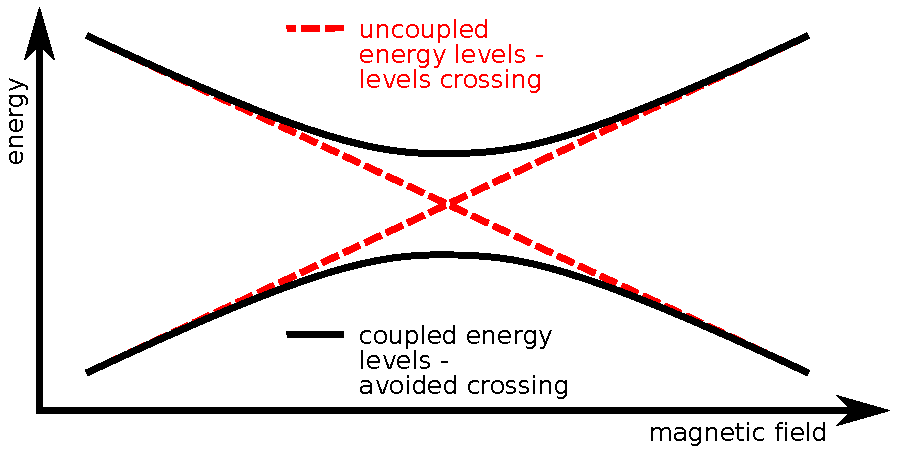
\includegraphics[width=0.9 \textwidth]{/figures/theory/LACs.pdf}
                \caption[Leval anti crossings]{A generic example of level anti crossings. In red, the uncoupled states can be seen while in black, the energy states including the coupling are shown.}
                \label{figure:theory:LAC}
            \end{figure}
            This means that the coupling leads to a mixing of the states if the magnetic field is in the region of the LAC. Effectively, the coupling thus changes the occupatinal numbers of the uncoupled states over time. See section \ref{HPSabre} for how this effect can be used to hyperolarize samples.
    \section{NMR}
    Nuclear Magnetic Resonance (NMR) is a technique that emerged in 1946 with the discovery of the absortion properties of nuclei irradiated with electromagnetic waves resonant to their larmor frequencies \cite{ResonanceAbsorption}. The subsequent observation of signal from those previously excited nuclei \cite{rabi_space_1937,purcell_resonance_1946-1,bloch_nuclear_1946}, known as free induction decay (FID) paved the road to the now well established method which in the beginning was primarily used in chemistry for structural analysis of molecules and chemical kinetics \cite{perrin_application_1990,lipkind_computer-assisted_1988}. This chapter will describe te theoretical basis of that technique keeping in mind that many theoretical aspects are already covered in section \ref{theory:section:nucleiSpins} and will only be briefly mentioned. 
        \subsection{Larmor frequency}
        \label{section:theory:larmorFrequency}
            Inside an external magnetic field $B_0$, a magnetic dipole $\mu$ will precess with a frequency
            proportional to $B_0\cdot \mu$. This also applies to charged particles with a spin $S\neq0$ and thus
            a magnetic moment $\mu\neq0$. The precession is a result of the torque $\mu\times\vec B$
            excerted on the magnetic dipole moment.
            \begin{equation}
                f_L=\frac{\omega}{2\pi} = \frac{\gamma}{2\pi}\cdot B
            \end{equation}
        \subsection{Fourier transform, signal and signal to noise}
        \label{chapter:theory:fourierTransform}
        To analyze the acquired FIDs and echos, they're usually fourier transformed leading to a frequency analysis of the signal. This is achieved using the well known formula \cite{farrar_pulse_2012}
            \begin{equation}
            F(\omega) = \int^{\infty}_{-\infty}t \exp(-i\omega t)dt
            \end{equation}
            Note that the signal received is usually mixed with the center frequency of the NMR machine as the carrier frequency leading to the rotating frame frequencies being observed in the FID/echo. The frequency axis is subsequently shifted to provide absolute frequencies again.
            The signal consists of both the pure signal and additional noise from different sources. These include thermal noise, environmental noise and different forms of intrinsic electronics noise \cite{noauthor_henry_nodate}.
            If signal is low compared to noise levels, signal averaging can be applied to improve SNR. As signal increases with the number of scans n while noise does so only with $\sqrt n$ due to its random direction, n averages will improve the SNR by $n/\sqrt{n} = \sqrt{n}$ if other factors stay unchanged \cite{edelstein_intrinsic_1986}. 
        \subsection{Chemical shift}
            The larmor frequency of nuclei in NMR is largely governed by $B_0$ and $\mu$, but other factors do influence it on a more subtle scale. The most prominent effect besides the Zeeman splittings is the chemical shift which originates in the shielding of $B_0$ by the electrons' magnetic dilpoles surrounding the nucleus or molecule and is visible in the spectra \cite{gottlieb_nmr_1997}.  The shielding thus generally leads to a shift of precession frequency, where the chemical shift though is calculated as the relative frequency quota towards another known sample's reference frequency:
            \begin{equation}
                \delta = \frac{\nu_{sample} - \nu_{reference}}{\nu_{reference}}
            \end{equation}
            To have a field independent value for the chemical shift which to a good approximation scales linearly with the field, it is usually expressed in ppm of the center frequency.
        \subsection{J-coupling}
        In addition to the change in field by the electrons dipoles, the nucleis' magnetic dipoles inside one molecule will also interact. The interaction can be conveyed either directly or via the electrons' spins. The direct interaction is neglectable in liquids due to fastly rotating spins that average to zero. The indirect interaction via the electrons can also lead to a frequency shift resulting in multiplets usually on scales smaller than the chemical shifts, i.e. in the $\SI{}{\hertz}$ range 
        J couplings can be measured by evaluating the evolution of nuclei phases under the coupling using 2d-NMR spectra \cite{ottiger_measurement_1998}.
        \subsection{Flip angle}
            An external, on-resonant magnetic field will cause the magnetization of an ensemble of spins to flip by an angle $\alpha$ known as the flip angle (FA). A FA of $\mathrm n\cdot 270 \deg + 90 \deg$ with $n \in \mathbb{N}$ will rotate the magnetizatioh to the transverse plane perpendicular to the magnetic field resulting in an FID. Pulses of $\mathrm n\cdot 180 \deg$ will keep the magnetization aligned with the magnetic field or invert it, therefore not resulting in a FID or echo. All other FAs will produce a linear combination of the two cases. Note that in case of a \SI{180}{\degree} pulse, relaxation occurs along the z-axis despite the lack of NMR signal. The FA is defined as the time integral over the coil voltage with a coil specific calibration factor:
            \begin{equation}
                FA = A_c \int_{t=0}^{T_p}{V(t)dt}
            \end{equation}
            This means that, if the coil has been calibrated for one pulse form, e.g. a simple box pulse 
            \begin{equation}
                V(t) = A\sin{\omega_{RF} t + \phi_0} u(t)u(t-T_p)
            \end{equation}
            with duration $T_{RF}$ and heaviside function $u(t)$, every other pulse's FAs with arbitrarily shaped amplitude $A(t)$ can be calculated from that. This of course excludes effects like relaxation during pulsing \cite{wang_factors_2006}, which can be relevant especially for long pulses and also not considering hardware limitations on the coils concerning maximum voltage or wattage.
        \subsection{Shimming}
            As the field generated by the superconductor will not be perfectly homogeneous in itself and the samples introduce changes in magnetic susceptibility that further disturb the magnetic field, shimming, i.e. the retrospective homogenization of the field, plays an important role in NMR and MRI. Different order shims are differentiated reffering to the order of the polynomial they resemble e.g. for a linear shim in x direction
            \begin{equation}
                B(x) = B_0 + B_{gr} * x.
            \end{equation}
            Additionally, especially linear shims, or magnetic field gradients are used for spatial encoding in MRI applications \ref{section:theory:magneticGradient}.
        \subsection{A simple NMR experiment}
        The most basic experiment in NMR is the exposure of a spin ensemble to a $\SI{90}{\degree}$ RF pulse and subsequent readout. This will flip the magnetization by $\SI{90}{\degree}$ which will precess around the z axis afterwards with its Larmor frequency $\omega_L$. Using a coil\ref{materialsMethods:coils} mounted around the sample, the alternating field caused by the rotating magnetization will induce a current driving the resonant circuit (eq). \ref{equation:theory:maxwell}. That signal - FID or echo - can be recorded as the voltage over the resonant circuit. It can be described by a dampened sine wave
            \begin{equation}
                S(t) = S_0 \sin((\omega - \omega_0)  t + \phi) \exp(-\tfrac{t}{T_2})
            \end{equation}
            where $\omega$ is the larmor frequency of the observed particle, $\omega_0$ is the center frequency of the scanner and $T_2^*$ is the effective dephasing time constant (see \ref{chapter:theory:relaxation}). The phase $\phi$ varies depending on the axis of rotation chosen for the first pulse. Mostly, x- or y-pulses are used rotating the magnetization around the respective axis and resulting in phase shifts of \SI{90}{\degree} (x, y, -x, -y). As described in the NMR section (\ref{chapter:theory:fourierTransform}), the signal can then be fourier transformed and will give insight into local environments of the nuclei, i.e. their chemical shifts, the couplings they experience and also their relaxation rates (if experiments are repeated with different timings). 
        \subsection{Relaxation}
        \label{chapter:theory:relaxation}
        After being deflected from its thermal equilibrium, the magnetization tends to return to that equilibrium state. That process is called $T_1$ relaxation or spin-lattice relaxation and is an exponential decay (figure \ref{theory:figure:relaxation}, middle). In addition, the transverse magnetization decays with a time constant called $T_2$ (figure \ref{theory:figure:relaxation}, left) that is usually much smaller than $T_1$ \cite{levitt_spin_nodate}. $T_2$ relaxation occurs because of different magnetic fields experienced by the individual spins leading to a dephasing of the signal. That can be due to direct or indirect interaction between the spins ($T_2$) and also due to magnetic field inhomogenieties of different kinds. Both effects are combined are described by an effective relaxation constant $T_2^*$ \cite{chavhan_principles_2009}.
            \begin{figure}
                \centering
                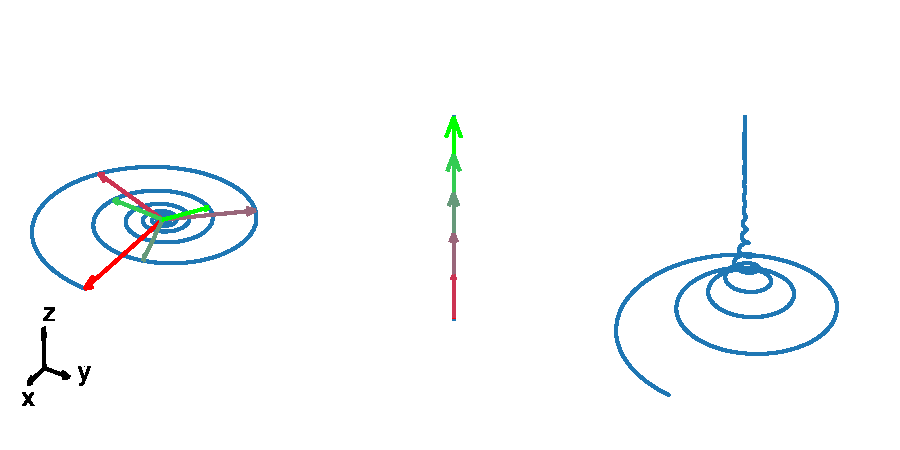
\includegraphics[width=0.9\textwidth]{/figures/theory/relaxation.pdf}
                \caption[Relaxation in NMR]{Exemplary plots of the T1 and T2 relaxation after a \SI{90}{\degree} FA shown via the magnetization and its temporal development. On te left, the magnetization in the xy-plane is shown with six arrows indicating equal timesteps. In the center, equal timesteps for the z-magnetization are shown. On the right, both cases are combined to show the overall magnetization. Note that generally, T1 is larger than T2 (here a factor of 40 difference). There are only few special cases where this won't hold.}
                \label{theory:figure:relaxation}
            \end{figure}
        \subsection{Inversion recovery and spin echos}
            $T_1$ times of a sample can be maesured using inversion recovery experiments. This is usually a \SI{180}{\degree} pulse followed by \SI{90}{\degree} pulses at different evolution times $T_{ev}$. Alternatively, the \SI{90}{\degree} angle can be replaced by many, smaller angle pulses. That will make aquisition faster, but has to be considered in the interpretation of the data. For non-uniform samples, $T_1$ values can also be acquired with a spatial encoding using steady state sequences \cite{scheffler_t1_2001}.
            The dephasing of the signal can be fast, but a part, defined by the difference between T2 and T2* can be regained through inversion of the magnetization. The inversion can be induced by a \SI{180}{\degree} RF pulse, in steady state measurements, often smaller pulses are used. The "resurrected" signal is called "echo". Multiple echos can be recorded if multiple inversion pulses are applied, but different effects effectively reduce the signal in the course of the recording:
            \begin{itemize}
                \item Diffusion and convection will reduce the efficiency of the signal recovery because both coupling environments and external fields will change due to the change in position.
                \item Pure $T_2$ deacay is not recoverable and will reduce the signal
                \item $T_1$ relaxation reduces the overall x/y magnetization and thus the signal amplitude exponentially.
            \end{itemize}
            In a steady state equilibrium, these effects can be inhibited mostly, which makes steady state sequences the tool of choice for imaging where nucleus density shall be observed (or $T_1$/ $T_2$) \cite{nitz_contrast_1999}.
        \subsection{2D-NMR}
        In addition to the standard NMR spectrum that can get difficult to interpret when many or large molecules are present and multiple nuclei contribute to the signal, a 2D NMR method called COSY emerged in 1976 \cite{}. As the name suggests, are not recorded and shown in the usual 1D-plot, but in a 2D plot adding a dimension to display more information. The method is very similar to the MRI method described in chapter \ref{theory:section:MRI} although here, no field gradients are necessary yet: the second dimension simply shows the development of certain nuclei under specific evolution times that are defined by the pulse sequence. By varying the evolution times and fourier transforming the spectra in the second spatial dimension, the frequency of the coupling will be indicated \cite{finster_two-dimensional_1980}.
        \subsection{Field Gradients}
            \label{section:theory:magneticGradient}
            For different purposes it is beneficial to not only have the homogeneous $B_0$ field, but to also introduce magnetic field gradients. Generally, these are additional fields ideally oriented exactly along the primary magnetic field's direction that change with one of the spatial dimentions x, y and/or z. The most common, minimum requirement for imaging are linear gradients, i.e. fields that in- or decrease linearly with one spatial direction. More complex gradients \cite{littin_development_2018} are mostly used for shimming \cite{kim_regularized_2002} but also for advanced imaging sequences such as radial sequences such as the 'stack of stars' sequence \cite{burdumy_one-second_2016}. Generation of magnetic field gradients is usually achieved through normal conductors of specifically tailored geometries. Gradient strengths and ramping speeds are limited by the specific absorption rates (SAR) that are defined by the IEC standard \cite{noauthor_iec_nodate} as spatially or temporally quickly changing magnetic fields can cause neuronal stimulation in living tissue.
    \section{MRI}
    \label{theory:section:MRI}
        A huge addition to the world of NMR was the invention of spatially resolved sample maps, i.e. imaging. It was made possible through the clever use of gradients and largely resembles 2D-NMR sequences.
        \subsection{MRI in Medicine}
        As a non-invasive, non-ionizing imaging method, MRI has become important in many parts of the medical field for example neurology \cite{frisoni_clinical_2010}, oncology \cite{padhani_dynamic_2002}, cardiology \cite{constantine_role_2004} or urology \cite{stoianovici_mri_2007}. While the low polarization of nuclei make its sesitivity inferior to other imaging methods such as computed tomography, the nature of the signal generation allow for contrasts that differ vastly from other established methods. This uniqueness allows for superior imaging power in many cases despite the smaller sensitvity. In the following, a basic imaging sequence is described \cite{noauthor_wiley-vch_nodate}.
        \subsection{Magnetic field gradients}
        As described before, magnetic field gradients are used for shimming, but also for spatial encoding of the NMR signal. The latter is described in more detail in the following. Imaging sequences consist of RF pulses, magnetic field gradients and readout - all planned and aligned in a specific setting.
        \subsection{Spin echo sequence}
            A spin echo sequence consists of a excitation pulse (often \SI{90}{\degree}) followed by a train of \SI{180}{\degree} pulses. Every 180\SI{}{\degree} pulse leads to a inversion of the magnetization along the z-axis (as soon as the steady state is reached) \cite{brown_mri_2005}. The time thus, the pulse train induces an echo train that can be recorded by the receive coils as each inversion causes the spins of the ensemble to rephase according to the specifications in the relaxation section. This means that the time limiting factor for each signal acquisition is $T_2$. 
        \subsection{Gradient echo sequence}
            A gradient echo sequence uses an excitation pulse (ususally smaller \SI{90}{\degree}) to generate the initial x-y-magnetization, but relies on additional gradients to actively de- and rephase the magnetization in the following \cite{brown_mri_2005}. The RF pulses to invert magnetization used in the spin echo are dropped. This has the disadvantage that $T_2^*$ decay is the time limiting factor for acquisition though compensated by a generally faster acquisition because the dephasing itself can be quicker than the intrinsic relaxation. This reduces echo times and thus overall acquisition time.
        \subsection{Slice selection}
            The first step in most imaging methods is to excite a slice of the sample to select the first spatial dimension. To do so, a magnetic field gradient - mostly in z direction - is applied to the sample. 
            \begin{equation}
                B_z(z) = B_{z,max} * \frac{z}{z_{max}}
            \end{equation}
            This means that the frequency bandwidth together with the gradient strength are relevant parameters for the slice thickness $\Delta z$. It is given by 
            \begin{equation}
                \Delta f = \gamma G_z \Delta z
            \end{equation}
            where $G_z$ is the gradient strength in \SI{}{\tesla\per\meter}.
            Radiofrequency pulses have a limited frequency bandwidth. Thus, with the z-gradient turned on, they will affect only nuclei within a slice of the thickness defined by
            \begin{equation}
                \Delta z = \Delta f_{pulse} \cdot \frac{1}{\gamma G_z}.
            \end{equation}
             It has to be kept in mind that this does not necessarily guarantee that nuclei outside the prepared slice do not contribute to the signal. Movement of parts of the sample such as convectional flow or diffusion can lead to signal artifacts. Furthermore, the following pulses in the sequence have to be carefully designed to not generate FIDs or echos of their own that are not related to the originally selected slice.
        \subsection{Frequency encoding}
            During readout, a field gradient can be turned on to encode the second spatial dimension. Considering a positive x-gradient, the nuclei at higher x values will then generate a higher frequency than the ones at lower x values.
            \begin{equation}
                f(x) = \gamma B_0 + \gamma G_x \cdot x
            \end{equation}
            Note that the naming convention calling the gradient an x-gradient does not imply a field in x direction. A perfect x-gradient has magnetic z-components only which vary along the x-axis. By sampling the signal and fourier transforming it, a molecule positioned at high x will generate signal at higher frequencies, i.e. at higher x in the frequency plot, than the same molecule positioned further to the right. The output is thus a projection of the slice onto the x-axis.
            Often, the recording of the echos is called sampling k-space as the fourier transform of the recorded data is the image in position-space. As this approach of the problem can be confusing in my opinion, I will try to keep going at it from the other, the position-space side.
        \subsection{Phase encoding}
            Generating an encoding for the third spatial dimension is not quite as straightforward.  To do so, a third gradient in a third dimension perpendicular to the two others, a y-gradient, is necessary.  Due to the redundancy that would occur if both x- and y-gradients were switched on at once (equifrequency circles), that gradient cannot simply be turned on during readout though.  It is instead used to change the phase of the signal the nuclei generate depending on the y-position in the sample. It generates an additional phase that depends on gradient strength and switch on time:
            \begin{equation}
                \phi = \gamma G_y t
            \end{equation}
            That means that the gradient strength needs to be varied to satisfy the sampling conditions for the frequencies generated, i.e. the freuquency encoding scheme is run multiple times with different phase encoding gradient field strengths set up to be running before it. That way, if the fourier transformed data for each phase encoding step, i.e. each frequency encoded line, is sorted by gradient strength and fourier transformed in the second dimension, the frequency generated by the changing phase will indicate the position in y direction. That means that each phase encoding step generates a k-space line that is shifted in the $k_y$ direction.
            \begin{figure}
                \includegraphics[width=0.9\textwidth]{/figures/theory/imagingScheme.pdf}
                \centering
                \caption[k-space Graph]{An abstract visualization of an imaging sequence. On the left, the gradients in frequency and phase encoding gradients are displayed over the course of one phase encoding step. For each of these steps, the pahse encoding gradient's strength ist varied. The usual display of the encoding steps in k-spaceis displayed on the right. Each repetition of the scheme on the left corresponds to one line in $k_x$ direction on the right.}
            \end{figure}
        \subsection{Adiabatic field switching}
        To generate more signal while keeping some advantages of a low field like higher absolute homogeniety, prepolarization can be used. A field that is larger than the field used in readout is switched on for a certain time before readout. The timing is largely influenced by T1 as the relaxation constant defines how long it takes for the sample to be in its new thermal equilibrium. The switching of the field can be performed quickly or slowly where quick switching means at switching times $t_s << T_1$ (adiabatically). 
    \section{Hyperpolarization}
        The main limitation of NMR and MRI is the low thermal polarization at room temperature and the currently generatable magnetic fields. The states follow the Boltzmann distribution \cite{canet_para-hydrogen_2006} which, for each energy state $E_i$, dictates
        \begin{equation}
            N_i = \exp{\frac{E_i}{k_B T}}
        \end{equation}
        For energy differences between two states that are small compared to the thermal Energy, the polarization can be expressed as follows:
        \begin{equation}
            P = {N_+-N_-}{N} = \tanh\left(\frac{\hbar \gamma B}{2 k T }\right)
            \label{equation:theory:polarization}
        \end{equation}
        This means, that even at the relatively high field strengths that can be generated in the spectrometers and MR imagers (order of \SI{10}{\tesla}), only a small fraction of the spins effectively contribute to the overall signal. Figure \ref{figure:theory:boltzmannDistribution} shows this shematically and for perfect hyperolarization. Note the size of the energy splitting compared to the total energy that differ by five orders of magnitude. In clinically relevant MRI machines that mostly operate at \SI{1.5}{\tesla} or \SI{3}{\tesla}, that means that a maximum of 1 in $10^6$ nuclei effectively contribute to the signal.
        \begin{figure}
            \centering
            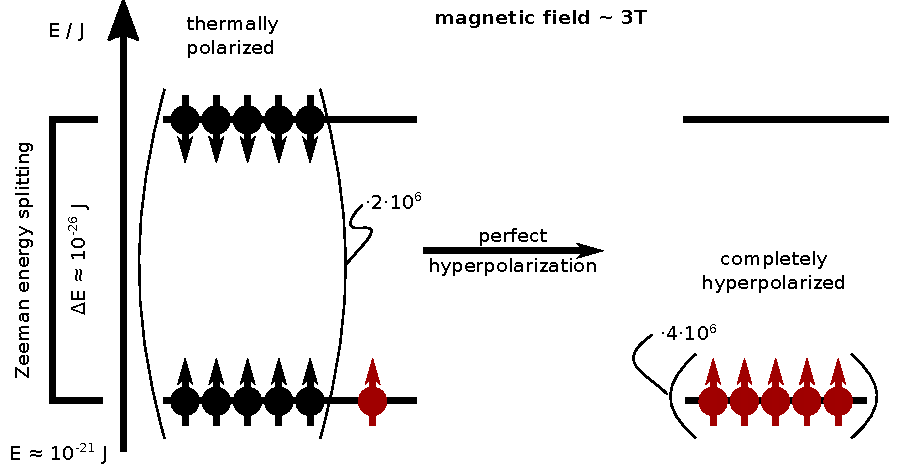
\includegraphics[width=0.9\textwidth]{/figures/theory/hyperpolarizationScheme.pdf}
            \caption[Hyperpolarization scheme]{Hyperpolarization can provide the means to drop all, or at least a lot more than in the thermally polarized case, of the spins to the lower energy level. That way, the overall magnetization and thus the signal observed is a lot higher than in ther thermally polarized case. The graph shows the case of perfect hyperpolarization of 1H at \SI{3}{\tesla}, which of course does not represent reality. At the fields currently used in clinical routine, only about one in 100000 spins effectively contributes to the signal.}
            \label{figure:theory:boltzmannDistribution}
        \end{figure}
        \subsection{Dynamic nuclear polarization}
        As the gyromagnetic ratio of electrons is much higher than that of any nucleus (factor of $10^{3}$ compared to protons), dynamic nuclear polarization (DNP) uses electrons at low temperatures and high fields to generate large initial polarization\cite{berliner_spin_1976}. The polarization is then transferred to specific nuclei by \si{\giga\hertz} microwave irradiation \cite{bajaj_dynamic_2011} that induces transitions in the spin system of nucleus and electron that is artificially generated by the addition of free radicals. The low temperatures lead to a freezing of the sample and microwaves are applied to it in that frozen state. For administration to a specimen or patient, the frozen sample then needs to be quickly melted and transferred \cite{johannesson_dynamic_2009}, usually in controlled magnetic environments \cite{} to prevent fast relaxation. The samples can show high polarizations close to unity but are usually limited by decay during the relatively long delivery times. Efforts building faster transport mechanisms have greatly reduced these times but they stay in the range of tens of seconds.
        \subsection{Hyperpolarization of noble gases}
        Noble gases such as 3He or 129Xe can be hyperpolarized by optical pumping \cite{middleton_mr_1995,oros_hyperpolarized_2004}. To do so, usually lasers are focused onto an optical cell through which the gas flows. The hyperpolarization is induced via the polarization of electron spins. An alkali metal, often Rubidium \cite{hersman_large_2008}, serves as a receptor for the laser induced optical pumping and subsequently hyperpolarizes the nuclei of the noble gas by spin exchange interactions \cite{walker_spin-exchange_1997}. Hyperpolarized gases are primarily used in lung imaging, but other uses e.g. in liquid state NMR or MRI by gas dissolution are not precluded \cite{duhamel_xenon-129_2001}.
        \subsection{Brute force hyperpolarization}
        As equation \ref{equation:theory:polarization} indicates, there are two main factors influencing polarizatoin: Magnetic field and temperature. It is not an option to freeze the objects to be measured of course, as strong polarization effects occur only close to absolute zero temperatures at the magnetic fields we can currently generate effectively. A viable alternative is to hyperpolarize a frozen tracer at high fields, thawing it and administering it to the subject \cite{hirsch_brute-force_2015}. Here, in contrast to DNP, no free radicals are necessary to generate the HP and - depnding on the relaxation constants in the field and temperature regime - no or less harmful additives than the free radicals for DNP are necessary. This makes a faster and mor lossles transfer of the sample to the subject possible. The high polarization generated on 1H can then be transfered to x-nuclei e.g. by passing the sample through low fields (< \SI{10}{\milli\tesla}). The transfer is driven by thermal mixing \cite{goldman_overview_2008} of the two spin species.
        \subsection{Parahydrogen induced Hyperpolarization}
            Parahydrogen is the singlet state of the hydrogen molecule, i.e. the antisymmetric mixed up/down state. Hydrogen molecules occur in one of the four states
            \begin{equation}
                 \begin{aligned}
                    T_+ &= |\uparrow\uparrow\rangle\\
                    T_0 &= \frac{1}{\sqrt{2}}\left(|\uparrow\downarrow\rangle + |\downarrow\uparrow\rangle\right)\\
                    T_- &= |\downarrow\downarrow\rangle\\
                    S &= \frac{1}{\sqrt{2}}\left(|\uparrow\downarrow\rangle - |\downarrow\uparrow\rangle\right)
                 \end{aligned}
            \end{equation}
            where T indicates the triplet state with overall spin I = 1 and S the singlet state with I = 0. At room temperature, the four states are almost equally occupied as thermal Energy is large compared to rotational energies of the molecule\todo{better wording}\cite{green_theory_2012-1}:
            \begin{equation}
                \frac{N_{ortho}}{N_{para}} = \frac{\sum_{J=even}(2J+1)\exp\left(-\frac{J(J+1)\Theta_R}{T}\right)}{3\sum_{J=odd}\left(2J+1\right)\exp\left(-\frac{J(J+1)\Theta_R}{T}\right)}
            \end{equation}
            which is $\tfrac{1}{3}$ plus terms depending on the ratio of thermal energy and rotational energy constant of the molecule. J is the rotational quantum number, $\Theta_R$ is the rotational energy constant of parahydrogen\cite{noauthor_orthohydrogen_1935}. At room temperature, the rotational energies can almost be neglected compared to thermal energy and the fraction is 1:3. Approaching absolute zero, the fraction of pH2 rises towards the pure pH2 state (see figure \ref{figure:theory:ph2Fraction}). At temperatures used to generate parahydrogen in this work, around \SI{21}{\kelvin}, the pH2 fraction is already close to 1.
            The conversion of oH2 to pH2 and back is forbidden quantum mechanically due to the change in angular momentum that would change the symmetry of the wavefunction \cite{minaev_spin_1995}. Therefore, conversions are only possible if different molecules collide and their nuclei interact or the rotational magnetic momentum interacts with one of the nuclei, which is both improbable and thus slow. To be able to generate pH2 fast and in large quantities, additional interaction needs to be introduced that catalyzes the conversion. Both charcoal catalysts and ironoxide have been proposed \cite{dechent_proton_nodate}. The catalyst creates field gradients on the scale of the hydrogen molecule which enables spin mixing of ortho and para states\cite{minaev_spin_1995} and thus a much faster conversion. This means that, at liquid helium temperatures which were used in this work, parahydrogen can be enriched to almost \SI{100}{\%}, a liquid nitrogen generator would enrich it to about 50 - \SI{60}{\%} \cite{zhuzhgov_low-temperature_2018}.
            As parahydrogen itself is a spin 0 particle, it is MR-invisible. Its ordered state can be used though to polarize other molecules, often referred to as substrate molecules.
            \begin{figure}
                \centering
                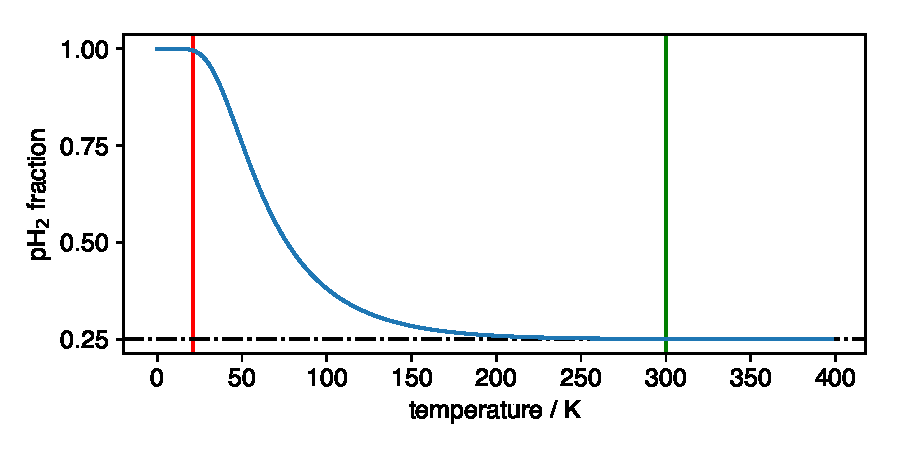
\includegraphics[width=0.9\textwidth]{/figures/theory/parahydrogenFraction.pdf}
                \caption[Parahydrogen fraction]{The equilibrium poplulation of the para hydrogen state. The dashed line shows the high temperature limit of 3:1. The green line indicates room temperature, where the limit is almost reached. The red line indicates the temperature at which parahydrogen was generated in this work, \SI{21}{\kelvin}.}
                \label{figure:theory:ph2Fraction}
            \end{figure}
            The initial density matrix of parahydrogen can be described by
            \begin{equation}
                \sigma_0^{pH_2} = \frac{1}{4} \hat 1 - c_0(\hat{I}_1\hat{I}_2)
            \end{equation}
            with the individual spins' operators denoted by 1 and 2 \cite{green_theory_2012-1} and the constant $c_0$ scaling with the fraction of $pH_2$ in the initial gas mixture:
            \begin{equation*}
                c_0=(4f_p-1)/3.
            \end{equation*}
            The evolution of the states is then described by the evolution of the density matrix under the J couplings with the target nuclei and other surrunding nuclei. 
        \subsubsection{Pasadena \& PHIP}
        The first parahydrogen induced polarization (PHIP) experiments were performed at the CIT in Pasadena \cite{bowers_parahydrogen_1987-2}, and later named after it (Pasadena/Altadena). These experiments used parahydrogen to hydrogenate a molecule first and then applied pulse sequences or field shuttling to transfer the hydrogens spin order to other nuclei. Mostly, 13C-labeled molecules were used as recipients of the spin order and susequent polarization. Figure \ref{} visualizes the hyperpolarization procedure. To make hyperpolarization possible, the parahydrogen needs to be added to the molecule pairwise, but have to be magnetically distinct after addition \cite{eisenberg_parahydrogen-induced_1991}. That means that after the addition, the symmetry of the added hydrogen molecule must be broken to be able to transfer the spin order. This usually happens alredy through the asymmetry of the receptor molecule and the different couplings of each added hydrogen atom to the nuclei of the molecule. Recently, the method has been extended and is now also used to hyperpolarize molecules that are more biologically relevant such as 13C labeled pyruvate \cite{cavallari_metabolic_2019}.
        \subsubsection{Sabre hyperpolarization}
        \label{HPSabre}
            The Sabre method was developed in 2009 \cite{adams_reversible_2009-2} for pyridine as a substrate and an Ir-based catalyst.
            In Sabre, the molecule to be hyperpolarized is not hydrogenated, but is in contact with the parahydrogen via the for a certain contact time $t_c$. The transfer of spin order can happen spontaneously at the right fields \cite{atkinson_spontaneous_2009-1} where socalled level-anti-crossings (LACs) occur. In addition, hyperpolarized susbtrate can also be generated at fields far from these LACs using RF-irradiation \cite{pravdivtsev_spin_2014, knecht_quantitative_2019} and can also be enriched using selective RF-pulses \cite{knecht_re-polarization_2018-1}. The system can be described by time evolution in bound and unbound state where the bound state implies non zero couplings between ph2 and at least some of the substrate spins.
            \begin{figure}
                \centering
                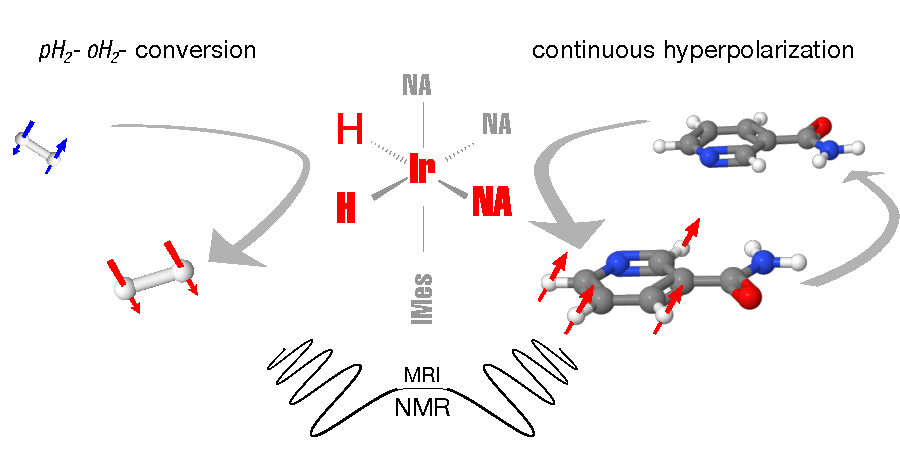
\includegraphics[width=0.9\textwidth]{/figures/theory/sabreScheme.pdf}
                \caption[Sabre scheme]{The mechanism used in Sabre using nicotinamide as an exemplary molecule. On the left, parahydrogen is converted to its ortho state, thus spin order is lost. On the right, nicotinamide is hyperpolarized by the transfer of that order.}
            \end{figure}
            To describe the time evolution of the bound system, the density matrix has to be evolved under the couplings present in the complex that forms when both parahydrogen and substrate are bound to, and thus coupled via, the catalyst \cite{}. The necessary hamiltonian is formed by the Zeeman term and all the relevant couplings (in the rotating frame notation):
            \begin{equation}
                \begin{aligned}
                    \mathcal{H}& = \mathcal{H}_z + \mathcal{H}_J \\
                        & =\-2\pi\gamma B_0 \sum_n{(1-\delta_n)\hat{I}_{nz}} + \sum_{n<m} -2\pi J_{nm}(\hat{I}_{nx}\hat{I}_{mx} + \hat{I}_{nx}\hat{I}_{mx}+ \hat{I}_{ny}\hat{I}_{my} + \hat{I}_{nx}\hat{I}_{mx})
                \end{aligned}
            \end{equation}
            Additionally, the binding time that depends on temperature and diffusion constants of the solvent has a strong influence on the effective coupling the nuclei experience.
            Hyperpolarized signal occurs at different points: The substrate itself is hyperpolarized, and that is both in bound and free form, i.e. after detatching from the catalyst. The forms can be differentiated by hteir different chemical shifts. At usual concentrations, where a surplus of target substrate is present, the free form will exceed the bound form drastically. Additionally, the hydrogen will be in a ortho state and hyperpolarized after polarization has been transferred to the target molecule. It can also be seen in the $^1H$ spectrum.
            For $^{15}N$, only one resonance is observed for free and bound form, respectively. Here, as with $^1H$, the free form prevails the bound form under the concentrations used in the usual experiments and so do the respective signals.
        \section{Hardware}
            As hardware plays an important role in this work, I also want to provide a bit of theoretical insight into some of the technologies used in this work.
            \subsection{Field generation}
                Fields are generated by either current flown conductors or superconductors. Both have ad- and disadvantages and are chosen according to requirements (see ref{methods}). Magnetic field is generated according to the fourth Maxwell equation
                \begin{equation}
                    label{equation:theory:maxwell}
                    \vec\nabla\times\vec B = \mu_0\vec j+\mu_0\epsilon_0\frac{\partial\vec E}{\partial t}
                \end{equation}
                where $\vec j$ is the electric current generating the magnetic field together with changes in the electric field \cite{b.i._bleaney__b._bleaney_electricity_nodate}. For the static field of conductor, the current is the main mechanism for field generation and is described by the Biot-Savart-law.
            \subsubsection{Normal conductors}
                A normal conductor has the great advantage of room temperature operatiion simplifying its setup and use enormously. The disadwantage is that the conductor will heat due to its finite resistance. That heating can be so large that melting of the conductor occurs or, in the less dramatic case, deformations happens due to heat expansion or softening. Usually, copper is chosen for its low electric resistance of \SI{1.72e-8}{\ohm\meter}(reducing heat generation) and at the same time high thermal conductivity \SI{380}{\watt\per\m\per\kelvin}(increasing heat dissipation) \cite{schofield_f._h._thermal_1925}.
            \subsubsection{Superconductors}
            Superconductors are a special form of conductors that show electric resistances of exactly zero below a certain critical temperature $T_c$ discovered 1911 \cite{onnes_resistance_nodate}. Generally, the superconductors need to be cooled from room temperature to a few \SI{}{\kelvin} to show this property, modern alloys so called high temperature superconductors can, under certain conditions, raise that limit to about \SI{200}{\kelvin} \cite{drozdov_conventional_2015}. Superconductors can be made of different, rather exotic materials but also more common substances such as graphene can show superconducting properties. Different superconductors show different critical Temperatures and mechanical properties often restricting their use to certain fields. Microscopically, inside the superconductors, so called cooper pairs are forming \cite{bardeen_theory_1957}. These pairs of two electrons travel resistance free through phonon coupling, i.e. the deformation of the surrounding lattice caused by one electron distribution and the related energy loss is regained \SI{100}{\percent} by a second. That way, completely lossless movement of electrons is possible in the compound.
            \subsection{Magnetic susceptibility and shielding}
                The magnetic field generated by a current flow or a changing electric field is described by the magnetic field strength $\mat H$ which describes the magnetic field with no material present. The actually relevant size for experimental purposes is the magnetic flux density $B$ which adds to the magnetic field strength the magnetization $M$ of materials exposed to the magnetic field strength $H$.
                \begin{equation}
                    \vec{B} = \mu \vec{H} = \mu_0 \mu_r \vec{H} = \mu_0(1+\chi) \vec{H}
                \end{equation}
                where $\chi$ is the magnetic susceptibility \cite{schenck_role_1996}, the quantity mostly mentioned in NMR and MRI. Ususally $B$ is the unit intended when talking about magnetic fields.
                In many cases, as for example for air, $B$ and $H$ are almost the same as the relative permeability \cite{kriz_magnetic_1996} $\mu_r$ is only 0.35 ppm \cite{cullity_introduction_2008}. For water, it is already about a factor 10 higher, i.e. $\mu_r$ = 2~ppm . 
                This means that, where susceptibility changes occur in materials, magnetization and thus magnetic field change. These changes cause field inhomogenieties posing a problem for NMR and MRI where a more homogenous field $B_0$ is always preferred. Materials are grouped by their susceptibilities \cite{b.i._bleaney__b._bleaney_electricity_nodate}:
                Substances with a large, positive $\chi$ are called ferromagnetic, they get magnetized in the direction of the external field and the magnetization can surpass the field strength of the external field. External field and magnetization aren't usually linearly correlated for ferromagnets, when all magnetic moments in the material are aligned a plateau is reached. Usually, these materials follow a magnetization hysteresis when the external field changes value and sign. Furthermore, ferromagnets do not necessarily return to their unmagnetized state if H returns to 0 (remanence).
                Paramagnetic and diamegnetic substances show a much smaller magnetization, where paramgnetic substances nuclear momenta, as ferromagnetic ones align parallel to the magnetic field ($\chi>0$) and diamagnetic antiparallel ($\chi$ < 0).
                Shielding of external magnetic fields can make use of the fact that the high susceptibility of some materials leads to a bundling of magnetic field lines, i.e. a volume surrounded by that material can have a strongly reduced magnetic flux density and thus a lower magnetic field \cite{mager_magnetic_1970}.
            \subsection{Oscillating circuit}
                A coil for usage in NMR or MRI usually consists of oscillatory circuits made up of a capacitor and an inductance. Inside a ascillatory circuit, energy can be stored in the forms of electric field and electric current. The two forms of energy are constantly converted into each other, i.e. the capacitor is charged by the current coming from the coil and in turn generates a phase shifted countering current. The freuqency of this coversion can be calculated considering the following differential equations:
                \begin{equation}
                    \begin{aligned}
                        -L\frac{dI}{dt} &= \frac{Q}{C} \\
                        L\frac{d^2I}{dt^2} + \frac{I}{C} &= 0
                    \end{aligned}
                \end{equation}
                as the voltages of coil - that is proportional to the change in current according to Faradays law - and the capacitor - that depends on capacitance and charge - need to be equal at all times. The solution of this simplified case resulting in a ordinary second order differential equation with no linear term is simply a undampened oscillation:
                \begin{equation}
                    I(t) =  A \cdot \cos(\omega t) + \phi 
                \end{equation}
                where $f= \frac{1}{\omega} = \frac{1}{2\pi\sqrt{LC}}$ which means that by changing capacitance and inductance in a resonant circuit, the resulting resonance frequency can be changed \cite{rao_electronic_2011}. Moreover, capacitance and inductance sizes can be adapted in opposite directions depending on the purpose of operation.
                Of course, in realistic cases, the oscillation is dampened by ohmic resistance of the components and radiation losses.
            \subsection{Birdcage coils}
            Commercially available volume resonators are often manufactured in the birdcage design. The advantage of that design is the \todo{fin}
            \subsection{Nyquist theorem}
            Especially in the low field spectrometer case, where no frequency mixing was performed as is usually the case at the MRI's much higher frequencies, one had to keep in mind sampling theorems to ensure a proper signal coverage. A signal needs to be sampled at a minimum sampling frequency \cite{shannon_mathematical_1948}
                \begin{equation}
                    f_{s} = 2 f_{sig}
                \end{equation}
                if signals with a maximum frequency of $f_{sig}$ are expected. If the sampling frequency is lower than that, aliasing effects will occur, i.e. fold ins in the fourier transform will show up.
                Another option would be to limit the bandwidth towards the lower end by a high pass filter and use this a priori knowledge to prevent the aliasing.
            \subsection{Operational amplifiers}
                Operational amplifiers have been used to amplify the signal of the fluxgate magnetic field sensor. Amplification is necessary because of the large output range of $\pm$ \SI{10}{\volt} in combination with the high resolution in the low field regime. Operational amplifiers are a rather complex network of transistors that show a behavior similar to what is described in the following. The ideal operational amplifier amplifies the incoming signal to infinity on the positive input, to $-\inf$ on the negative input and has an infinite input impedance as well. This is not true in practice, but very high voltages (limited by the supply voltage) are produced at the output if a small voltage is applied to either of the inputs. With the gain $A_{opa}$, the output voltage is thus described by
                \begin{equation}
                        \label{equation:theory:OPAvoltage}
                    U_{out} = A_{opa}(V_+ - V_-)
                \end{equation}
                That is why operational amplifiers need to be driven in some kind of feedback mode (figure \ref{figure:theory:opAmp}) as otherwise even very small voltage differences on the input cause a saturation of the output. In this mode, the output is fed back to one of the inputs, most of the time via resistors, to generate a defined output voltage that depends on the input voltage of the complete setup, $U_{in}$. The socalled inverting opamp was used in this work, is shown in figure \ref{figure:theory:opAmp} and will be described in more detail now.
                \begin{figure}
                    \includegraphics[width=0.9\textwidth]{/figures/theory/opAmp.pdf}
                    \caption[Operational amplifier]{An operational amplifier in an inverting setup. The amplification of the input voltage $U_{in}$ is directly given by the ratio of the resistors, $R_2/R_1$.}
                \end{figure}
                By connecting the output to the negative input, a loop is formed in which the voltages add to zero. This tells us that
                \begin{equation*}
                    U_{opa} = U_{out} - U_- = U_{R_2}
                \end{equation*}
                Additionally, as, as soon as the negative input starts to differ from the positive one, the output reacts and drives it back. That way, there is a virtual ground on the negative input (marget with a red dot in figure \ref{figure:theory:opAmp}).
                This can also be shown by calculating the voltage $U_-$:
                \begin{equation}
                    U_- = U_{in} + U_{R_1} = U_{R_2} + U_{out}
                \end{equation}
                which, considering $R_1$ and $R_2$ are a voltage divider due to the lack of current trough the opamp, this can be written as
                \begin{equation}
                    U_{-} = U_{out} \frac{R_1}{R_1+R_2} + U_{in} \frac{R_2}{R_1+R_2}
                \end{equation}
                and, if combined with equation \ref{equation:theory:OPAvoltage}, gives the output voltage
                \begin{equation}
                    U_{out} = -U_{in} \frac{A_{opa}R_2}{R_1+R_2 + A_{opa}R_1}
                \end{equation}
                which, for large $A_{opa}$ present in all operational amplifiers simplifies to the Resistor ratio.
                \begin{equation}
                    U_{out} = -U_{in}\frac{R_2}{R_1}
                \end{equation}
                This also makes sense phenomenologically: by this setup, $U_{+}$ and $U_{-}$ are kept at the same level, i.e. the negative input is a virtual ground, as the output is fed back to the negative input and any pertubance that causes a differential voltage between the two inputs will regulate itsself by applying a corresponding voltage to the negative input until equilibrium is restored \cite{huijsing_operational_2017-1}.
                This is especially helpful as the accuracy of the resistors is the limiting factor of the amplification's accuracy, i.e. by choosing the resistors carefully, the aplification can be set very accurately.
            \subsection{Frequency filters}
                For reducing noise when interested in certain regions of the frequency spectrum only, frequency filters can be used. They differ in the steepnes of the cutoff frequency, socalled order, and the transmission efficiency (no Filter is completely lossless at the unblocked frequencies). The easiest frequency filter is just a combination of a capacitor and a resistor or a inductance and a resistor as shown in figure \ref{figure:theory:frequencyFilter}. Using the impedances of inductance and capacitor
                \begin{equation*}
                    Z_C = -i\frac{1}{\omega C}
                \end{equation*}
                \begin{equation*}
                    Z_L = {i\omega L}
                \end{equation*} 
                The output voltage $U_o$can then be described as a function of input voltage $U_{i}$ and these two impedances:
                \begin{equation}
                    U_o = \frac{Z_c}{Z_R + Z_C} U_i
                \end{equation}
                with the signal frequency $\omega$. The cutoff frequency of the filter $f_0$ can then be described for both the RC-filter by
                \begin{equation}
                    f_0^{RC} = \frac{1}{2\pi R C}
                \end{equation}
                and the RL-filters:
                \begin{equation}
                    f_0^{RL} = \frac{R}{2\pi L}
                \end{equation}
                where the arrangement of the components defines whether it is a low or a high pass filter. These filters are the simplest form of frequency filters of first order and show a boundary drop of \SI{20}{\deci\bel} per frequency decade. Higher order filters can be used where more sharply defined cutoff frequencies are necessary but usually come with drawbacks in the linearity of the transmit band especially close to the cutoff frequency (ripple). These can be constructed by combining multiple frequency filters serially or by designing more complex filters such as the Chebyshev filter, a LC filter wih n stages. Figure \ref{figure:theory:frequencyFilter} demonstrates the effect of first and second order filters on the signal at different frequencies.
            \begin{figure}
                \label{figure:theory:frequencyFilter}
                \centering
                \includegraphics[width=0.9\textwidth]{/figures/theory/frequencyFilters.pdf}
                \caption[Frequency filters]{Transfer function over frequency for the different types of filters mentioned in the text. Cutoff frequencies are shown for the filters. At the frequency value of 10, a first order high and low pass filter are shown for the same cutoff frequency (i.e. same L/C and R values) in purple colors. Further to the right, a shifted first order filter (C/L * 10) and a second order filter are shown in shades of red.}
            \end{figure}
            \subsection{Flow and flow resistance}
                Pressure differences above liqids or in gases create flow from high to low pressure area. These flows are important in the setups used here and will be shortly described as a function of the pressure creating them under simplified conditions. The flow is described by the navier stokes equations \cite{sochi_flow_2013}.
                Flowing speeds are generally limited by the flow resistance. This resistance is easily described if the flow is through a tube and can be considered laminar. Generally, the flow rate Q is given by 
                \begin{equation}
                    Q=\frac{p_2-p_1}{R}
                \end{equation}
                where R is the reynolds number corresponding to electrical resistance and that depends on $\eta$, the viscosity of the fluid and the flow resistance of the connecting vessel. For example, for a solid tube of radius r and length l, the reynolds number is given by \cite{jeffrey_particle_1965}
                \begin{equation}
                    R=\frac{8\eta l}{\pi r^4}
                \end{equation}
                Because of the much lower viscosity of gases that stems from their lower density, gas flow is generally higher than fluid flow at otherwise unchanged conditions.
